% !TeX program = xelatex
\documentclass[a4paper,10pt]{article}

% ============================================================================
% កញ្ចប់បណ្ណាល័យ (Packages) – តាមលំនាំ NGS Preah Krasang (ls_plan.tex)
% បរិបទ៖ គ្មានស្លាយ LCD និងគ្មានម៉ាស៊ីនគិតលេខ — ប្រើសន្លឹកកិច្ចការសិស្ស (ស-ខ្មៅ) និងក្ដារខៀនជាគោល
% ============================================================================
\usepackage[a4paper, left=0.95cm, right=0.95cm, top=0.85cm, bottom=0.92cm, footskip=0.52cm]{geometry}
\usepackage{amsmath}
\usepackage{unicode-math}
\usepackage{fontspec}
\usepackage{array, longtable, multirow, colortbl}
\usepackage[table]{xcolor}
\usepackage{enumitem}
\usepackage{pifont}
\usepackage{fancyhdr}
\usepackage{tikz}
\usetikzlibrary{calc, arrows.meta, angles, quotes, decorations.markings, decorations.pathreplacing, patterns, babel}

\makeatletter
\let\@expl@@@mark@update@singlecol@structures@@\relax
\makeatother

\providecommand{\NGSFindFonts}{%
  \IfFileExists{C:/Windows/Fonts/cambria.ttc}{%
    \def\NGSSysPath{C:/Windows/Fonts/}%
    \def\NGSUserPath{C:/Users/KIT/AppData/Local/Microsoft/Windows/Fonts/}%
  }{%
    \IfFileExists{./fonts/KhmerOSsiemreap.ttf}{\def\NGSSysPath{./fonts/}\def\NGSUserPath{./fonts/}}{%
    \IfFileExists{../fonts/KhmerOSsiemreap.ttf}{\def\NGSSysPath{../fonts/}\def\NGSUserPath{../fonts/}}{%
    \IfFileExists{../../fonts/KhmerOSsiemreap.ttf}{\def\NGSSysPath{../../fonts/}\def\NGSUserPath{../../fonts/}}{%
    \IfFileExists{../../../fonts/KhmerOSsiemreap.ttf}{\def\NGSSysPath{../../../fonts/}\def\NGSUserPath{../../../fonts/}}{%
    \IfFileExists{../../../../fonts/KhmerOSsiemreap.ttf}{\def\NGSSysPath{../../../../fonts/}\def\NGSUserPath{../../../../fonts/}}{%
    \IfFileExists{../../../../../fonts/KhmerOSsiemreap.ttf}{\def\NGSSysPath{../../../../../fonts/}\def\NGSUserPath{../../../../../fonts/}}{%
    \IfFileExists{../../../../../../fonts/KhmerOSsiemreap.ttf}{\def\NGSSysPath{../../../../../../fonts/}\def\NGSUserPath{../../../../../../fonts/}}{%
      \def\NGSSysPath{../../../../../../../fonts/}\def\NGSUserPath{../../../../../../../fonts/}%
    }}}}}}}%
  }%
}
\NGSFindFonts

\setmathfont[Path={\NGSSysPath}, FontIndex=1, Scale=1.02]{cambria.ttc}
\defaultfontfeatures{Ligatures=TeX}

\setmainfont[
  Path={\NGSUserPath}, Extension=.ttf, Script=Khmer,
  BoldFont={KhmerOSsiemreap}, BoldFeatures={FakeBold=1.8},
  ItalicFont={KhmerOSsiemreap}, ItalicFeatures={FakeSlant=0.25},
  BoldItalicFont={KhmerOSsiemreap}, BoldItalicFeatures={FakeBold=1.8, FakeSlant=0.25}
]{KhmerOSsiemreap}

\newfontfamily\muol[Path={\NGSUserPath}, Extension=.ttf, Script=Khmer]{KhmerOSmuollight}
\newfontfamily\TimesEn[Path={\NGSSysPath}, Extension=.ttf, Scale=1.00, BoldFont={timesbd}, ItalicFont={timesi}, BoldItalicFont={timesbi}]{times}
\newfontfamily\NagaBold[Path={\NGSUserPath}, Extension=.ttf]{AKbalthom Naga Bold}
\newfontfamily\CalibriFont[Path={\NGSSysPath}, Extension=.ttf]{calibri}
\newfontfamily\Tacteing[Path={\NGSUserPath}]{TACTENG.TTF}
\newfontfamily\CourierBullet[Path={\NGSSysPath}, Extension=.ttf]{cour}
\newcommand{\wcirc}{{\CourierBullet\fontsize{9.5pt}{11pt}\selectfont o}}

\XeTeXlinebreaklocale "km"
\XeTeXlinebreakskip = 0pt plus 1pt minus 0.1pt

\definecolor{stepgray}{HTML}{D9D9D9}
\definecolor{headgray}{HTML}{F2F2F2}
\definecolor{boxgray}{HTML}{D9D9D9}
\definecolor{darkred}{HTML}{C00000}
\definecolor{red5e}{HTML}{FF0000}

\pagestyle{fancy}
\fancyhf{}
\renewcommand{\headrulewidth}{0pt}
\fancyfoot[R]{\CalibriFont\fontsize{11pt}{13pt}\selectfont\thepage}

\setlength{\parindent}{0pt}
\setlength{\parskip}{0pt}
\setlength{\tabcolsep}{3.8pt}

\newcolumntype{L}[1]{>{\raggedright\arraybackslash}p{#1}}
\newcolumntype{C}[1]{>{\centering\arraybackslash}p{#1}}

\newcommand{\en}[1]{{\TimesEn #1}}
\newcommand{\enbf}[1]{{\TimesEn\textbf{#1}}}
\newcommand{\unit}[1]{\,\text{\en{#1}}}
\newcommand{\fiveE}[1]{{\NagaBold\fontsize{9.5pt}{13pt}\selectfont\textcolor{red5e}{#1}}}
\newcommand{\timenote}[1]{\textcolor{darkred}{\textit{#1}}}
\newcommand{\redsub}[1]{\textcolor{darkred}{#1}}
\newcommand{\graybox}[1]{\colorbox{boxgray}{\strut\hspace{2pt}#1\hspace{2pt}}}
\newcommand{\ditem}{\tikz[baseline=-0.5ex]\fill (0,0.42ex) -- (0.42ex,0) -- (0,-0.42ex) -- (-0.42ex,0) -- cycle;\hspace{0.3em}}
\newcommand{\cnum}[1]{{\fontsize{10.5pt}{12pt}\selectfont\ding{\numexpr181+#1\relax}}\hspace{0.15em}}
\newcommand{\cfig}[1]{\par\vspace{3pt}{\centering #1\par}\vspace{3pt}}
\newcommand{\stepheader}[1]{\multicolumn{3}{|c|}{\cellcolor{stepgray}\muol #1} \\* \noalign{\hrule height 0.4pt}}
\newcommand{\khmflourish}{{\Tacteing\fontsize{36pt}{14pt}\selectfont\raisebox{-5pt}{3}}}

% ============================================================================
% ម៉ាក្រូគូសរូប TikZ ស-ខ្មៅ ១០០% សម្រាប់មេរៀន ៣.២.១ & ៣.២.២ (PCT1)
% ============================================================================

% ១. E1 Engage: អន្ទាក់ឯកតា 45m នៃ 1km និងអន្ទាក់ភាគរយចំណេញ (ទំ.៣១-៣២)
\newcommand{\figEngagePCTA}{%
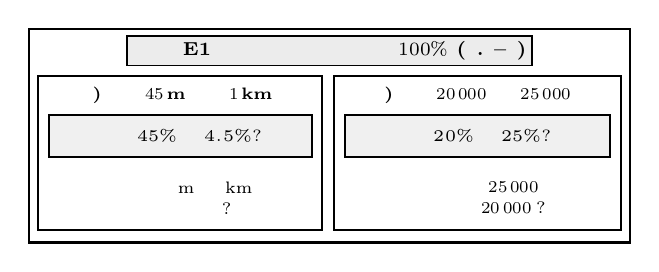
\begin{tikzpicture}[x=0.96cm, y=0.92cm, every node/.style={font=\scriptsize, text=black}]
  \draw[black, line width=0.95pt] (0,0) rectangle (7.95,2.95);
  \node[fill=gray!15, draw=black, line width=0.6pt, inner sep=2pt, font=\fontsize{6.8pt}{8.5pt}\selectfont\bfseries] at (3.975,2.65) {បេសកកម្ម \en{E1}៖ ច្រកឯកតារួម និងយុថ្កាគោលថ្លៃដើម $100\%$ (ទំ.៣១–៣២)};

  \draw[black, line width=0.8pt] (0.12,0.18) rectangle (3.88,2.30);
  \node[font=\fontsize{6.0pt}{7.8pt}\selectfont\bfseries] at (2.00,2.04) {១) ចម្ងាយ $45\unit{m}$ ធៀបនឹង $1\unit{km}$};
  \draw[black, line width=0.75pt, fill=gray!12] (0.26,1.18) rectangle (3.74,1.76);
  \node[font=\fontsize{5.9pt}{7.6pt}\selectfont] at (2.00,1.47) {ស្មើនឹង $45\%$ \;ឬ\; $4.5\%$?};
  \node[align=center, font=\fontsize{6.0pt}{7.6pt}\selectfont] at (2.00,0.62) {តើអាចប្រៀបធៀប $\unit{m}$ និង $\unit{km}$\\ដោយមិនប្ដូរឯកតាបានទេ?};

  \draw[black, line width=0.8pt] (4.04,0.18) rectangle (7.83,2.30);
  \node[font=\fontsize{6.0pt}{7.8pt}\selectfont\bfseries] at (5.935,2.04) {២) ទិញអាវ $20\,000\text{៛}$ លក់ $25\,000\text{៛}$};
  \draw[black, line width=0.75pt, fill=gray!12] (4.18,1.18) rectangle (7.69,1.76);
  \node[font=\fontsize{5.9pt}{7.6pt}\selectfont] at (5.935,1.47) {ចំណេញ $20\%$ \;ឬ\; $25\%$?};
  \node[align=center, font=\fontsize{6.0pt}{7.6pt}\selectfont] at (5.935,0.62) {តើចែកនឹង\textbf{ថ្លៃលក់} $25\,000\text{៛}$\\ឬចែកនឹង\textbf{ថ្លៃដើម} $20\,000\text{៛}$?};
\end{tikzpicture}}

% ២. E2 POE 2: របារយុថ្កាគោលថ្លៃដើម 100% (ចំណេញ vs ខាត)
\newcommand{\figAnchorBarPCTA}{%
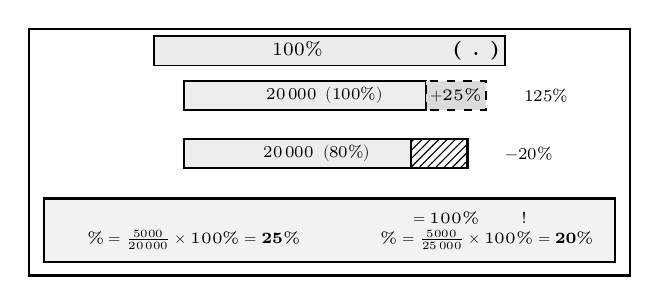
\begin{tikzpicture}[x=0.96cm, y=0.92cm, every node/.style={font=\scriptsize, text=black}]
  \draw[black, line width=0.95pt] (0,0) rectangle (7.95,3.40);
  \node[fill=gray!15, draw=black, line width=0.6pt, inner sep=2pt, font=\fontsize{6.8pt}{8.5pt}\selectfont\bfseries] at (3.975,3.10) {របារយុថ្កាគោលថ្លៃដើម $100\%$៖ ប្រៀបធៀបចំណេញ និងខាត (ទំ.៣២)};

  % Case 1: Profit
  \node[anchor=west, font=\fontsize{6.1pt}{7.8pt}\selectfont] at (0.18,2.48) {\textbf{ករណីចំណេញ៖}};
  \draw[black, line width=0.8pt, fill=gray!14] (2.05,2.28) rectangle (5.25,2.68);
  \node[font=\fontsize{6.0pt}{7.6pt}\selectfont] at (3.65,2.48) {ថ្លៃដើម $20\,000\text{៛} \;(100\%)$};
  \draw[black, line width=0.8pt, dashed, fill=gray!28] (5.25,2.28) rectangle (6.05,2.68);
  \node[font=\fontsize{5.8pt}{7.4pt}\selectfont] at (5.65,2.48) {$+25\%$};
  \node[anchor=west, font=\fontsize{6.0pt}{7.6pt}\selectfont] at (6.15,2.48) {លក់ $125\%$};

  % Case 2: Loss
  \node[anchor=west, font=\fontsize{6.1pt}{7.8pt}\selectfont] at (0.18,1.68) {\textbf{ករណីខាត៖}};
  \draw[black, line width=0.8pt, fill=gray!14] (2.05,1.48) rectangle (5.05,1.88);
  \node[font=\fontsize{6.0pt}{7.6pt}\selectfont] at (3.55,1.68) {ថ្លៃលក់ $20\,000\text{៛} \;(80\%)$};
  \draw[black, line width=0.8pt, pattern=north east lines] (5.05,1.48) rectangle (5.80,1.88);
  \node[anchor=west, font=\fontsize{6.0pt}{7.6pt}\selectfont] at (5.90,1.68) {ខាត $-20\%$};

  % Rule box
  \draw[black, line width=0.75pt, fill=gray!10] (0.20,0.18) rectangle (7.75,1.06);
  \node[align=center, font=\fontsize{5.7pt}{7.4pt}\selectfont] at (3.975,0.62) {\textbf{ច្បាប់យុថ្កាគោល៖} ទាំងភាគរយចំណេញ និងខាត ត្រូវយក \textbf{ប្រាក់ថ្លៃដើម $= 100\%$} ជាភាគបែង!\\$\text{ចំណេញ}\% = \frac{5000}{20\,000}\times 100\% = \mathbf{25\%}$ \quad ខុសពី \quad $\text{ខាត}\% = \frac{5000}{25\,000}\times 100\% = \mathbf{20\%}$};
\end{tikzpicture}}

% ៣. E4 Worked Example: ទិញ-លក់រថយន្តពីរដំណាក់កាល (ទំ.៣២)
\newcommand{\figCarResalePCTA}{%
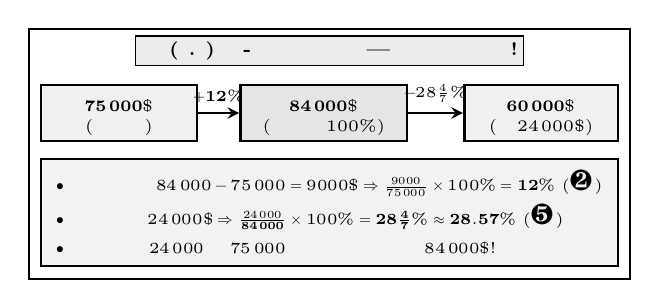
\begin{tikzpicture}[x=0.96cm, y=0.92cm, every node/.style={font=\scriptsize, text=black}]
  \draw[black, line width=0.95pt] (0,0) rectangle (7.95,3.45);
  \node[fill=gray!15, draw=black, line width=0.6pt, inner sep=2pt, font=\fontsize{6.6pt}{8.4pt}\selectfont\bfseries] at (3.975,3.15) {គំរូ (ទំ.៣២)៖ ទិញ-លក់រថយន្តពីរដំណាក់កាល — ប្ដូរយុថ្កាថ្លៃដើមថ្មី!};

  % Stage 1
  \draw[black, line width=0.8pt, fill=gray!12] (0.16,1.90) rectangle (2.22,2.68);
  \node[align=center, font=\fontsize{5.8pt}{7.4pt}\selectfont] at (1.19,2.29) {\textbf{ម្ចាស់ទី ១ ទិញ}\\$\mathbf{75\,000\$}$\\(ថ្លៃដើមទី ១)};

  \draw[->, >=stealth, line width=0.85pt] (2.24,2.29) -- node[above, font=\fontsize{5.6pt}{7.2pt}\selectfont]{$+\mathbf{12\%}$} (2.78,2.29);

  % Stage 2
  \draw[black, line width=0.85pt, fill=gray!20] (2.80,1.90) rectangle (5.00,2.68);
  \node[align=center, font=\fontsize{5.8pt}{7.4pt}\selectfont] at (3.90,2.29) {\textbf{ម្ចាស់ទី ២ ទិញ}\\$\mathbf{84\,000\$}$\\(ថ្លៃដើមថ្មី $100\%$)};

  \draw[->, >=stealth, line width=0.85pt] (5.02,2.29) -- node[above, font=\fontsize{5.5pt}{7.0pt}\selectfont]{$-28\frac{4}{7}\%$} (5.74,2.29);

  % Stage 3
  \draw[black, line width=0.8pt, fill=gray!12] (5.76,1.90) rectangle (7.79,2.68);
  \node[align=center, font=\fontsize{5.8pt}{7.4pt}\selectfont] at (6.775,2.29) {\textbf{លក់ចេញវិញ}\\$\mathbf{60\,000\$}$\\(ខាត $24\,000\$$)};

  % Calculations bottom box
  \draw[black, line width=0.75pt, fill=gray!10] (0.16,0.18) rectangle (7.79,1.66);
  \node[anchor=west, font=\fontsize{5.6pt}{7.3pt}\selectfont] at (0.24,1.32) {$\bullet$ \textbf{ដំណាក់ទី ១៖} ចំណេញ $84\,000-75\,000=9000\$ \Rightarrow \frac{9000}{75\,000}\times 100\% = \mathbf{12\%}$ (\cnum{2})};
  \node[anchor=west, font=\fontsize{5.6pt}{7.3pt}\selectfont] at (0.24,0.86) {$\bullet$ \textbf{ដំណាក់ទី ២៖} ខាត $24\,000\$ \Rightarrow \frac{24\,000}{\mathbf{84\,000}}\times 100\% = \mathbf{28\frac{4}{7}\%} \approx \mathbf{28.57\%}$ (\cnum{5})};
  \node[anchor=west, font=\fontsize{5.6pt}{7.3pt}\selectfont] at (0.24,0.42) {$\bullet$ \textbf{ប្រយ័ត្ន៖} ហាមចែក $24\,000$ នឹង $75\,000$ ព្រោះម្ចាស់ទី ២ ទិញក្នុងថ្លៃ $84\,000\$$!};
\end{tikzpicture}}

% ៤. E5 Diagnostic Options A-D
\newcommand{\figExitCardsPCTA}{%
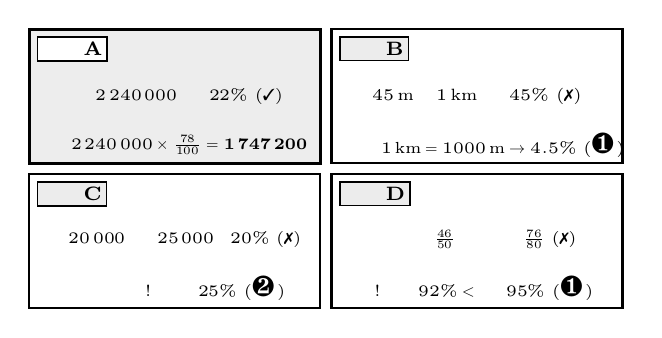
\begin{tikzpicture}[x=0.96cm, y=0.92cm, every node/.style={font=\scriptsize, text=black}]
  \draw[black, line width=1.1pt, fill=gray!14] (0,2.00) rectangle (3.85,3.85);
  \node[anchor=north west, fill=white, draw=black, line width=0.6pt, inner sep=1.8pt] at (0.10,3.75) {\textbf{ជម្រើស \en{A}}};
  \node[font=\fontsize{5.8pt}{7.5pt}\selectfont] at (1.925,2.92) {ម៉ូតូ $2\,240\,000\text{៛}$ ខាត $22\%$ (\ding{51})};
  \node[font=\fontsize{5.8pt}{7.5pt}\selectfont] at (1.925,2.25) {\textbf{លក់បាន} $2\,240\,000\times\frac{78}{100}=\mathbf{1\,747\,200\text{៛}}$};

  \draw[black, line width=0.9pt] (4.00,2.00) rectangle (7.85,3.85);
  \node[anchor=north west, fill=gray!15, draw=black, line width=0.6pt, inner sep=1.8pt] at (4.10,3.75) {\textbf{ជម្រើស \en{B}}};
  \node[font=\fontsize{5.9pt}{7.6pt}\selectfont] at (5.925,2.92) {$45\unit{m}$ នៃ $1\unit{km}$ ស្មើ $45\%$ (\ding{55})};
  \node[font=\fontsize{5.8pt}{7.5pt}\selectfont] at (5.925,2.25) {ភ្លេចប្ដូរ $1\unit{km}=1000\unit{m} \to 4.5\%$ (\cnum{1})};

  \draw[black, line width=0.9pt] (0,0) rectangle (3.85,1.85);
  \node[anchor=north west, fill=gray!15, draw=black, line width=0.6pt, inner sep=1.8pt] at (0.10,1.75) {\textbf{ជម្រើស \en{C}}};
  \node[font=\fontsize{5.8pt}{7.5pt}\selectfont] at (1.925,0.95) {ទិញ $20\,000\text{៛}$ លក់ $25\,000\text{៛}$៖ $20\%$ (\ding{55})};
  \node[font=\fontsize{5.8pt}{7.5pt}\selectfont] at (1.925,0.28) {ច្រឡំចែកនឹងថ្លៃលក់! ត្រូវជា $25\%$ (\cnum{2})};

  \draw[black, line width=0.9pt] (4.00,0) rectangle (7.85,1.85);
  \node[anchor=north west, fill=gray!15, draw=black, line width=0.6pt, inner sep=1.8pt] at (4.10,1.75) {\textbf{ជម្រើស \en{D}}};
  \node[font=\fontsize{5.8pt}{7.5pt}\selectfont] at (5.925,0.95) {ពិន្ទុខ្មែរ $\frac{46}{50}$ ខ្ពស់ជាងគណិត $\frac{76}{80}$ (\ding{55})};
  \node[font=\fontsize{5.8pt}{7.5pt}\selectfont] at (5.925,0.28) {ខុស! ខ្មែរ $92\% <$ គណិត $95\%$ (\cnum{1})};
\end{tikzpicture}}

\begin{document}
\fontsize{10pt}{15.2pt}\selectfont

% -------------------- ក្បាលកិច្ចតែងការ --------------------
\begin{center}
  {\muol\fontsize{11pt}{16pt}\selectfont ព្រះរាជាណាចក្រកម្ពុជា}\\[2pt]
  {\muol\fontsize{10pt}{15pt}\selectfont ជាតិ សាសនា ព្រះមហាក្សត្រ}\\[1pt]
  \khmflourish
\end{center}

\vspace{-24pt}
{\muol\fontsize{9.5pt}{12.5pt}\selectfont
មន្ទីរអប់រំ យុវជន និងកីឡា ខេត្តកំពង់ធំ\\
ការិយាល័យអប់រំ យុវជន និងកីឡា ស្រុកកំពង់ស្វាយ\\
អនុវិទ្យាល័យព្រះក្រសាំង}

\vspace{1pt}
\begin{center}
  {\muol\fontsize{10pt}{14pt}\selectfont កិច្ចតែងការបង្រៀន}
\end{center}
\vspace{0pt}

% -------------------- ព័ត៌មានទូទៅ --------------------
{\renewcommand{\arraystretch}{0.98}
\hspace*{3.1cm}%
\begin{tabular}{@{}l l L{11.0cm}@{}}
  - \hspace{0.35cm} មុខវិជ្ជា & : & គណិតវិទ្យា ថ្នាក់ទី៨ (ពីជគណិត) \\
  - \hspace{0.35cm} ចំណងជើងមេរៀន & : & មេរៀនទី៣៖ ទំហំសមាមាត្រ និងភាគរយ \\
  - \hspace{0.35cm} ចំណងជើងរង & : & ២.១. ភាគរយនៃបរិមាណមួយ និង ២.២. ប្រាក់ចំណេញ-ខាត (ទំ.៣១–៣៣ និងលំហាត់ \#3, \#5ខ-គ ទំ.៤០–៤១) \\
  - \hspace{0.35cm} រយៈពេល & : & ១ ម៉ោងសិក្សា (៥០ នាទី) \\
  - \hspace{0.35cm} បង្រៀនដោយ & : & ហុក ប៊ុនថែន \\
  - \hspace{0.35cm} កាលបរិច្ឆេទ & : & ថ្ងៃសៅរ៍ ទី២៨ ខែវិច្ឆិកា ឆ្នាំ២០២៦ \\
\end{tabular}

\vspace{2pt}

% -------------------- I. វត្ថុបំណង --------------------
\textbf{I.} {\muol វត្ថុបំណង}\\[1pt]
\hspace*{0.55cm}%
\begin{tabular}{@{}l l L{14.2cm}@{}}
  \wcirc \hspace{0.25cm} វិជ្ជាសម្បទា & : & សិស្សប្រាប់រូបមន្តសរសេរបរិមាណមួយជាភាគរយនៃបរិមាណមួយទៀតក្នុងឯកតារួម ($\frac{A}{B}\times 100\%$) ព្រមទាំងរូបមន្តគណនាភាគរយចំណេញ និងភាគរយខាតធៀបនឹងប្រាក់ថ្លៃដើម ($100\%$) ។ \\
  \wcirc \hspace{0.25cm} បំណិនសម្បទា & : & សិស្សប្ដូរឯកតាឱ្យដូចគ្នាមុនគណនាភាគរយ ប្រៀបធៀបពិន្ទុប្រឡងជាភាគរយ និងដោះស្រាយចំណោទប្រាក់ចំណេញ-ខាតមួយដំណាក់ និងពីរដំណាក់កាល (ទំ.៣១–៣៣) លើសន្លឹកកិច្ចការ ។ \\
  \wcirc \hspace{0.25cm} ចរិយាសម្បទា & : & សិស្សមានភាពម៉ត់ចត់ក្នុងការពិនិត្យឯកតា និងកំណត់យុថ្កាប្រាក់ថ្លៃដើមបានត្រឹមត្រូវក្នុងការគណនាជីវភាពប្រចាំថ្ងៃ ។ \\
\end{tabular}

\vspace{2pt}

% -------------------- II. សម្ភារៈឧបទេស --------------------
\textbf{II.} {\muol សម្ភារៈឧបទេស}\\[1pt]
\hspace*{0.55cm}$\bullet$ \hspace{0.35cm} សៀវភៅសិក្សាគោលគណិតវិទ្យាថ្នាក់ទី៨ (ទំ.៣១–៣៣, ៤០–៤១) ក្ដារខៀន ដីស និងសន្លឹកកិច្ចការសិស្ស ស-ខ្មៅ (\en{Worksheet\_PCT1} ទំព័រ ១–២ គ្មានស្លាយ \en{LCD})

\vspace{2pt}

% -------------------- III. វិធីសាស្រ្តបង្រៀន --------------------
\textbf{III.} {\muol វិធីសាស្រ្តបង្រៀន}\\[1pt]
\hspace*{0.45cm}%
\begin{tabular}{@{}l l L{14.85cm}@{}}
  $\bullet$ \hspace{0.25cm} គោលវិធី & : & សិស្សមជ្ឈមណ្ឌល (បង្រៀនតាមសន្លឹកកិច្ចការស៊ើបអង្កេត និងក្ដារខៀន គ្មាន \en{LCD}) \\
  $\bullet$ \hspace{0.25cm} យុទ្ធវិធីបង្រៀន & : & គំរូ \en{5Es} រួមបញ្ចូលច្រកឯកតារួម និងរបារយុថ្កាគោលថ្លៃដើម $100\%$ (\en{Reference-Base $100\%$ Anchor Bar}) \\
\end{tabular}
}

\vspace{2pt}

% -------------------- IV. ដំណើរការបង្រៀន --------------------
\textbf{IV.} {\muol ដំណើរការបង្រៀន}

\vspace{1pt}

\renewcommand{\arraystretch}{1.15}
\begin{longtable}{|L{5.50cm}|L{7.90cm}|L{4.80cm}|}
\hline
\rowcolor{headgray}
\multicolumn{1}{|c|}{\muol សកម្មភាពគ្រូ} &
\multicolumn{1}{c|}{\muol ខ្លឹមសារមេរៀន} &
\multicolumn{1}{c|}{\muol សកម្មភាពសិស្ស} \\
\hline
\endfirsthead
\hline
\endhead
\hline
\endfoot
\hline
\endlastfoot

% ==================== ជំហានទី១ (2min) ====================
\stepheader{ជំហានទី១ \enbf{(}រដ្ឋបាលថ្នាក់\enbf{)}}
$\bullet$ ពិនិត្យអវត្តមាន អនាម័យ និងសណ្ដាប់ធ្នាប់ថ្នាក់រៀន
&
$\bullet$ រដ្ឋបាលថ្នាក់ និងការរៀបចំដៃគូសិក្សា
&
$\circ$ ប្រធានថ្នាក់រាយការណ៍អវត្តមាន \\[3pt]

$\bullet$ ចែក \textbf{សន្លឹកកិច្ចការសិស្ស (\en{Worksheet\_PCT1})} ម្នាក់ ១ សន្លឹក (ផ្កាប់ទុកសិន)
&
$\bullet$ សន្លឹកកិច្ចការសិស្ស ស-ខ្មៅ (\en{Worksheet\_PCT1} ទំព័រ ១–២)
&
$\circ$ ទទួលសន្លឹកកិច្ចការ និងត្រៀមសម្ភារៈសរសេរ \\
\hline

% ==================== ជំហានទី២ (9min: <=3 + 3 + E1 3) ====================
\stepheader{ជំហានទី២ \enbf{(}កិច្ចការផ្ទះ \enbf{+} ទំនាក់ទំនងមេរៀនថ្មី\enbf{)}}
\ditem \textbf{កំណែកិច្ចការផ្ទះ ($\le 3\unit{min}$)} \timenote{(កុំសរសេរវែង)} \par
$\bullet$ ហៅសិស្ស ២ នាក់ឡើងសរសេរចម្លើយលំហាត់ \#8 និង \#13 (ទំ.៤១) លើក្ដារខៀន
&
{\centering\redsub{កំណែកិច្ចការផ្ទះមេរៀន ១.៣ (ទំ.៤០–៤១ \#6ឃ-ង, \#8, \#9, \#13)}\par} \par
$\bullet$ \textbf{\#6ឃ-ង និង \#8៖} ពិនិត្យផលគុណថេរ $xy = a$ និងសរសេរសមីការ $y = \frac{a}{x}$ \par
$\bullet$ \textbf{\#13៖} ដោះស្រាយចំណោទសមាមាត្រច្រាសតាម $x_1 y_1 = x_2 y_2$
&
$\circ$ ផ្ទៀងផ្ទាត់ និងកែតម្រូវចម្លើយក្នុងសៀវភៅកិច្ចការផ្ទះ \\[3pt]

\ditem \textbf{រំលឹកមេរៀនទាក់ទង (3min)} \par
$\bullet$ សួររហ័ស៖ ប្ដូរប្រភាគ $\dfrac{3}{4}$ និង $\dfrac{1}{5}$ ជាភាគរយ
&
{\centering\redsub{រំលឹកសញ្ញាណភាគរយ និងការប្ដូរឯកតារង្វាស់}\par} \par
$\bullet$ ប្ដូរប្រភាគជាភាគរយ៖ $\dfrac{3}{4}\times 100\% = 75\%$ \;;\; $\dfrac{1}{5}\times 100\% = 20\%$
&
$\circ$ ឆ្លើយរហ័សអំពីការប្ដូរប្រភាគជាភាគរយ \\[3pt]

$\bullet$ សួររហ័សបន្ត៖ ប្រាប់ទំនាក់ទំនងឯកតារង្វាស់ $1\unit{km} = ?\unit{m}$ និង $1\unit{kg} = ?\unit{g}$
&
$\bullet$ ប្ដូរឯកតា៖ $1\unit{km} = 1000\unit{m}$ \;;\; $1\unit{kg} = 1000\unit{g}$ \;;\; $1\unit{h} = 60\unit{mn}$
&
$\circ$ ឆ្លើយរហ័សអំពីការប្ដូរឯកតារង្វាស់ \\[3pt]

\fiveE{E1 - Engage (3min)} \timenote{(កុំទាន់ផ្ដល់ចម្លើយ)} \par
\ditem \textbf{«បេសកកម្មទីផ្សារ និងច្រកឯកតារួម»} \par
$\bullet$ ឱ្យសិស្សបើកសន្លឹកកិច្ចការទំព័រ ១ គូសធីកទស្សន៍ទាយលើសំណួរ ២
&
{\centering\redsub{បេសកកម្ម E1៖ អន្ទាក់ឯកតាខុសគ្នា និងអន្ទាក់ភាគបែងថ្លៃលក់}\par} \par
$\bullet$ \textbf{សំណួរ ១ (ទំ.៣១)៖} ចម្ងាយ $45\unit{m}$ ស្មើប៉ុន្មានភាគរយនៃ $1\unit{km}$ ($45\%$ ឬ $4.5\%$)? \par
$\bullet$ \textbf{សំណួរ ២៖} ទិញអាវថ្លៃ $20\,000\text{៛}$ លក់បាន $25\,000\text{៛}$ — តើចំណេញ $20\%$ ឬ $25\%$?
&
$\circ$ គូសធីកទស្សន៍ទាយលើសន្លឹកកិច្ចការទំព័រ ១ \\[3pt]

&
\cfig{\figEngagePCTA}
& \\[3pt]

$\bullet$ ស្រង់ចំនួនដៃសិស្សកត់លើក្ដារខៀន (មិនទាន់ប្រាប់ចម្លើយត្រូវ)
&
$\bullet$ ស្ថិតិទស្សន៍ទាយ៖ $45\%$ ទល់នឹង $4.5\%$ ; ចំណេញ $20\%$ ទល់នឹង $25\%$
&
$\circ$ លើកដៃបង្ហាញការទស្សន៍ទាយ \\
\hline

% ==================== ជំហានទី៣ (17min: E2 11m + E3 6m) ====================
\stepheader{ជំហានទី៣ \enbf{(}ខ្លឹមសារមេរៀនថ្មី\enbf{)}}
\fiveE{E2 - Explore (11min)} \par
$\bullet$ សរសេរចំណងជើងផ្នែកទី២ និងចំណងជើងរងលើក្ដារខៀន
&
\textbf{២. ភាគរយ — ២.១. ភាគរយនៃបរិមាណមួយ និង ២.២. ប្រាក់ចំណេញ-ខាត} (ទំ.៣១–៣៣)
&
$\circ$ កត់ចំណងជើងចូលសៀវភៅ \\[3pt]

\ditem \textbf{សកម្មភាព ១៖ ច្រកឯកតារួមលើភាគរយនៃបរិមាណ \en{POE 1} (5min, ទំ.៣១)} \par
$\bullet$ ឱ្យដៃគូប្ដូរឯកតាឱ្យដូចគ្នាមុនសរសេរប្រភាគភាគរយលើសន្លឹកកិច្ចការ ($45\unit{m}$ នៃ $1\unit{km}$ និងសិស្សស្រី $30$ នាក់ក្នុងថ្នាក់ $40$ នាក់)
&
{\centering\textbf{សកម្មភាព ១ (\en{POE 1})៖ ច្រកឯកតារួម (ទំ.៣១)}\par} \par
$\bullet$ $1\unit{km} = 1000\unit{m} \implies \dfrac{45}{1000}\times 100\% = \dfrac{45}{10}\% = \mathbf{4.5\%}$ (មិនមែន $45\%$ ទេ!) \par
$\bullet$ គំរូសិស្សស្រី (ទំ.៣១)៖ $\dfrac{30}{40}\times 100\% = \mathbf{75\%}$ (សិស្សប្រុស $= 100\%-75\% = \mathbf{25\%}$)
&
$\circ$ ប្ដូរឯកតាឱ្យដូចគ្នា និងគណនាភាគរយនៃបរិមាណលើសន្លឹកកិច្ចការ \\[3pt]

\ditem \textbf{សកម្មភាព ២៖ របារយុថ្កាគោលថ្លៃដើម $100\%$ \en{POE 2} (6min, ទំ.៣២)} \par
$\bullet$ ឱ្យដៃគូប្រៀបធៀបករណីទាំងពីរលើសន្លឹកកិច្ចការ៖ ករណីទី១ ទិញ $20\,000\text{៛}$ លក់ $25\,000\text{៛}$ ទល់នឹង ករណីទី២ ទិញ $25\,000\text{៛}$ លក់ $20\,000\text{៛}$
&
{\centering\textbf{សកម្មភាព ២ (\en{POE 2})៖ ប្រៀបធៀបភាគរយចំណេញ និងភាគរយខាត}\par} \par
$\bullet$ \textbf{ករណីទី ១ (ថ្លៃដើម $20\,000\text{៛}$)៖} ចំណេញ $5000\text{៛} \implies \dfrac{5000}{20\,000}\times 100\% = \mathbf{25\%}$ \par
$\bullet$ \textbf{ករណីទី ២ (ថ្លៃដើម $25\,000\text{៛}$)៖} ខាត $5000\text{៛} \implies \dfrac{5000}{25\,000}\times 100\% = \mathbf{20\%}$
&
$\circ$ រកឃើញថាប្រាក់ខុសគ្នា $5000\text{៛}$ ដូចគ្នា តែភាគរយខុសគ្នាព្រោះថ្លៃដើមខុសគ្នា! \\[3pt]

&
\cfig{\figAnchorBarPCTA}
& \\[3pt]

% --- E3 Explain (6min) ---
\fiveE{E3 - Explain (6min)} \par
\ditem \textbf{បង្គុំរូបមន្តសង្ខេប (ទំ.៣១–៣២) និងធនាគារហេតុផល (ផ្នែកទី២)} \par
$\bullet$ ឱ្យសិស្សបង្គុំប្រអប់រូបមន្ត \textbf{ភាគរយនៃបរិមាណមួយ} (ច្រកឯកតារួម)
&
$\bullet$ \textbf{ភាគរយនៃបរិមាណ (ឯកតារួម ទំ.៣១)៖} $\dfrac{A}{B}\times 100\%$ (បរិមាណ $A$ និង $B$ ត្រូវមានឯកតាដូចគ្នា!) ។
&
$\circ$ បំពេញប្រអប់រូបមន្តភាគរយនៃបរិមាណលើសន្លឹកកិច្ចការ \\[3pt]

$\bullet$ ឱ្យសិស្សបង្គុំប្រអប់រូបមន្ត \textbf{ភាគរយប្រាក់ចំណេញ និងភាគរយប្រាក់ខាត}
&
$\bullet$ \textbf{ភាគរយចំណេញ និងខាត (ទំ.៣២)៖} $\text{ចំណេញ}\% = \dfrac{\text{ប្រាក់ចំណេញ}}{\text{ប្រាក់ថ្លៃដើម}}\times 100\%$ \;;\; $\text{ខាត}\% = \dfrac{\text{ប្រាក់ខាត}}{\text{ប្រាក់ថ្លៃដើម}}\times 100\%$ ។
&
$\circ$ បំពេញប្រអប់រូបមន្តចំណេញ-ខាតលើសន្លឹកកិច្ចការ \\[3pt]

$\bullet$ សង្ខេប \textbf{ធនាគារហេតុផល \cnum{1}--\cnum{2}} អំពីច្រកឯកតារួម និងយុថ្កាគោលថ្លៃដើម
&
\textbf{ធនាគារហេតុផល \en{B\&W} (\cnum{1}--\cnum{5})៖} \par
\cnum{1} ច្រកឯកតារួម៖ ត្រូវប្ដូរបរិមាណទាំងពីរឱ្យមានឯកតាដូចគ្នាជាមុន មុនគណនាភាគរយ \par
\cnum{2} យុថ្កាថ្លៃដើម $100\%$៖ ភាគរយចំណេញ ឬខាត ត្រូវចែកនឹង\textbf{ប្រាក់ថ្លៃដើម}ជានិច្ច
&
$\circ$ ផ្ទៀងផ្ទាត់ហេតុផល \cnum{1}--\cnum{2} លើសន្លឹកកិច្ចការ \\[3pt]

$\bullet$ សង្ខេប \textbf{ធនាគារហេតុផល \cnum{3}--\cnum{5}} សម្រាប់រកថ្លៃលក់ និងការលក់បន្តពីរដំណាក់
&
\cnum{3} រូបមន្តថ្លៃលក់ពេលចំណេញ $p\%$៖ $\text{ថ្លៃលក់} = \text{ថ្លៃដើម}\times \frac{100+p}{100}$ \par
\cnum{4} រូបមន្តថ្លៃលក់ពេលខាត $q\%$៖ $\text{ថ្លៃលក់} = \text{ថ្លៃដើម}\times \frac{100-q}{100}$ \par
\cnum{5} លក់បន្តច្រើនដំណាក់៖ ដំណាក់នីមួយៗត្រូវយកថ្លៃទិញនៃដំណាក់នោះជាថ្លៃដើមថ្មី!
&
$\circ$ ផ្ទៀងផ្ទាត់ហេតុផល \cnum{3}--\cnum{5} លើសន្លឹកកិច្ចការ \\
\hline

% ==================== ជំហានទី៤ (20min: E4 10m + E5 10m) ====================
\stepheader{ជំហានទី៤ \enbf{(}ពង្រីកចំណេះដឹង និងវាយតម្លៃ\enbf{)}}
\fiveE{E4 - Elaborate (10min)} \par
\ditem \textbf{លំហាត់គំរូ៖ ទិញ-លក់រថយន្តពីរដំណាក់កាល (ទំ.៣២ — ផ្នែកទី៣)} \par
$\bullet$ ដឹកនាំដោះស្រាយ \textbf{គំរូទិញរថយន្ត $75\,000\$$ លក់ $84\,000\$$ រួចលក់បន្ត $60\,000\$$} ដោយកំណត់យុថ្កាថ្លៃដើមប្រចាំដំណាក់
&
{\muol លំហាត់គំរូ} \textbf{(ទំ.៣២ — រថយន្តពីរដំណាក់កាល)៖} \par
$\bullet$ \textbf{ដំណាក់ទី ១៖} ថ្លៃដើមទី១ $= 75\,000\$$, ចំណេញ $= 84\,000 - 75\,000 = 9000\$$ \par
$\implies \text{ចំណេញ}\% = \dfrac{9000}{75\,000}\times 100\% = \dfrac{900}{75}\% = \mathbf{12\%}$ (\cnum{2}) \par
$\bullet$ \textbf{ដំណាក់ទី ២៖} ថ្លៃដើមថ្មី $= 84\,000\$$, ខាត $= 84\,000 - 60\,000 = 24\,000\$$ \par
$\implies \text{ខាត}\% = \dfrac{24\,000}{84\,000}\times 100\% = \dfrac{2}{7}\times 100\% = \mathbf{28\frac{4}{7}\%} \approx \mathbf{28.57\%}$ (\cnum{5})
&
$\circ$ បំពេញតារាងដំណាក់ទាំងពីរ និងសម្រួលប្រភាគដោយដៃលើសន្លឹកកិច្ចការ \\[3pt]

&
\cfig{\figCarResalePCTA}
& \\[3pt]

$\bullet$ សួរសំណួរឆ្លុះបញ្ចាំង \textbf{\en{EIA Looking-Back} (៣០ វិនាទី)}
&
\textbf{\en{EIA Looking-Back}៖} «នៅដំណាក់ទី ២ ហេតុអ្វីយើងចែក $24\,000\$$ នឹង $84\,000\$$ មិនចែកនឹង $75\,000\$$?»
&
$\circ$ ឆ្លើយ៖ «ព្រោះម្ចាស់ទី ២ បានទិញរថយន្តក្នុងតម្លៃដើម $84\,000\$$!» \\[3pt]

% --- E5 Evaluate (10min) ---
\fiveE{E5 - Evaluate (10min)} \par
\ditem \textbf{ហ្វឹកហាត់ជាដៃគូលើ «ប្រតិបត្តិ ១ និង ២» (6min, ទំ.៣២–៣៣ — ផ្នែកទី៤-ក)} \par
$\bullet$ ឱ្យដៃគូធ្វើ \textbf{ប្រតិបត្តិទី ១ (ទំ.៣២ លើ — ពិន្ទុគណិតវិទ្យា $\frac{76}{80}$ និងភាសាខ្មែរ $\frac{46}{50}$)}
&
{\muol លំហាត់ប្រតិបត្តិ} \textbf{(ទំ.៣២ លើ និង ទំ.៣៣ លើ)៖} \par
$\bullet$ \textbf{១) ប្រតិបត្តិ (ទំ.៣២ — ប្រៀបធៀបពិន្ទុប្រឡង)៖} \par
គណិតវិទ្យា៖ $\dfrac{76}{80}\times 100\% = \mathbf{95\%}$ \;;\; ភាសាខ្មែរ៖ $\dfrac{46}{50}\times 100\% = \mathbf{92\%}$ \par
$\implies$ មុខវិជ្ជា\textbf{គណិតវិទ្យា}បានភាគរយខ្ពស់ជាង ($95\% > 92\%$)
&
$\circ$ គណនាភាគរយនៃមុខវិជ្ជាទាំងពីរ និងប្រៀបធៀប \\[3pt]

$\bullet$ ឱ្យដៃគូធ្វើ \textbf{ប្រតិបត្តិទី ២ (ទំ.៣៣ លើ — ម៉ូតូសុខថ្លៃ $2\,240\,000\text{៛}$ លក់ខាត $22\%$)} រួចប្ដូរសន្លឹកផ្ទៀង (\en{Pause-Review})
&
$\bullet$ \textbf{២) ប្រតិបត្តិ (ទំ.៣៣ — ម៉ូតូសុខខាត $22\%$)៖} \par
ប្រាក់ខាត $= 2\,240\,000\times \dfrac{22}{100} = 492\,800\text{៛}$ \par
ថ្លៃលក់ម៉ូតូ $= 2\,240\,000 - 492\,800 = \mathbf{1\,747\,200\text{៛}}$ (ឬ $2\,240\,000\times \frac{78}{100}$) (\cnum{4})
&
$\circ$ គណនាថ្លៃលក់ម៉ូតូ និងផ្ទៀងផ្ទាត់ជាមួយដៃគូ \\[3pt]

$\bullet$ បិទបេសកកម្ម \en{E1} និងឱ្យសិស្សវិនិច្ឆ័យ \textbf{ជម្រើស \en{A--D}} + \textbf{\en{Exit Check}} (4min)
&
$\bullet$ \textbf{បិទបេសកកម្ម \en{E1}៖} $45\unit{m}$ នៃ $1\unit{km}$ គឺ $4.5\%$ ; ទិញ $20\,000\text{៛}$ លក់ $25\,000\text{៛}$ គឺចំណេញ $25\%$ ។ \par
$\bullet$ \textbf{វិនិច្ឆ័យជម្រើស \en{A--D} លើសន្លឹកកិច្ចការ៖}
&
$\circ$ ផ្ទៀងចម្លើយ \en{E1} និងគូសវង់ជម្រើសត្រូវ \en{A} \\[3pt]

&
\cfig{\figExitCardsPCTA}
& \\[3pt]

$\bullet$ ពិនិត្យរហ័សលើសំបុត្រចេញនៅបាតសន្លឹកកិច្ចការ (៦០ វិនាទី)
&
$\bullet$ \textbf{\en{Exit Check}៖} ១) $300\unit{g}$ នៃ $2\unit{kg} = \frac{300}{2000}\times 100\% = 15\%$ ; ២) ទិញ $40\,000\text{៛}$ លក់ចំណេញ $15\% \implies 46\,000\text{៛}$ ។
&
$\circ$ បំពេញសំបុត្រចេញដោយខ្លួនឯង \\
\hline

% ==================== ជំហានទី៥ (<=2min) ====================
\stepheader{ជំហានទី៥ \enbf{(}កិច្ចការផ្ទះ \enbf{+} បណ្ដាំផ្ញើ\enbf{)}}
\timenote{ចំណាយពេលឱ្យតិចបំផុតកុំឱ្យលើស 2min} \par
$\bullet$ ណែនាំកិច្ចការផ្ទះនៅបាតសន្លឹកកិច្ចការ (សៀវភៅពុម្ព ទំ.៤០–៤១ លំហាត់ \#3 និង \#5ខ-គ)
&
{\centering{\muol កិច្ចការផ្ទះ} \textbf{(សៀវភៅគោល ទំ.៤០–៤១ លំហាត់ \#3(ក,ខ,គ,ឃ) និង \#5(ខ,គ))៖}\par} \par
$\bullet$ \textbf{លំហាត់ \#3 (ទំ.៤០)៖} សរសេរបរិមាណទី១ ជាភាគរយនៃបរិមាណទី២ (ប្ដូរឯកតារួមជាមុន!) \par
$\bullet$ \textbf{លំហាត់ \#5ខ-គ (ទំ.៤១)៖} គណនាភាគរយនៃបរិមាណ និងប្រាក់ចំណេញ-ខាតធៀបនឹងថ្លៃដើម
&
$\circ$ កត់ចំណាំលំហាត់ទំ.៤០–៤១ សម្រាប់ធ្វើនៅផ្ទះ \\[3pt]

$\bullet$ ផ្ដាំផ្ញើឱ្យអានមុន \textbf{២.៣. ការបញ្ចុះតម្លៃ និង ២.៤. បម្រែបម្រួលភាគរយ (ទំ.៣៣–៣៥)}
&
$\bullet$ \textbf{មេរៀនបន្ទាប់៖} អានមុន \textbf{២.៣. ការបញ្ចុះតម្លៃ និង ២.៤. បម្រែបម្រួលភាគរយ (ទំ.៣៣–៣៥)} ។
&
$\circ$ កត់ចំណាំមេរៀនបន្ទាប់ និងជម្រាបលាគ្រូ \\
\end{longtable}

\vspace{6pt}
\hfill
\begin{minipage}{10.5cm}
  {\centering
    ថ្ងៃសៅរ៍ ៤រោច ខែកត្តិក ឆ្នាំមមី អដ្ឋស័ក ពុទ្ធសករាជ ២៥៧០\\[2pt]
    កំពង់ស្វាយ, ថ្ងៃទី២៨ ខែវិច្ឆិកា ឆ្នាំ២០២៦\\[3pt]
    {\muol គ្រូបង្រៀន}\par}
  \vspace{28pt}
  \hfill{\muol ហុក ប៊ុនថែន}\hspace*{1.4cm}
\end{minipage}

\end{document}
